\chapter{Repository Deep Dive}
\section{Verilator Simulator}
\subsection{About}
The primary way to simulate SoCs' designed using the Chipyard framework is via Verilator simulations the directory for verilator is \mintinline{bash}{/path/to/chipyard/sims/verilator}.
A base/example simulation can be run by using \mintinline{bash}{make} in the verilator directory.
Custom Chipyard configs can be simulated by running \mintinline{bash}{make CONFIG=*your custom config*}.
Running the make command produces a simulator executable in the verilator directory.
For example, if your project name was ``TestConfig'', running \mintinline{bash}{make CONFIG=TestConfig} would create an executable called simulator-chipyard-TestConfig in the verilator directory.
Custom RISCV code can be run by using the command \mintinline{bash}{./simulator-chipyard-TestConfig /path/to/riscv/executable}.

\subsection{Generators}
\subsubsection{Chipyard Generator}
\subsubsection{SHA3 Accelerators}

\subsection{Custom Configurations}
Custom Configs can be created in the directory \mintinline{bash}{chipyard/generators/chipyard/src/main/scala/config/}.
For example, I created a new scala file called \file{NewTestConfig.scala} in the directory, allowing me to create a simulator from a class inside the NewTestConfig.scala file.
Example Configs can be found in  \file{RocketConfigs.scala} in the same directory.

% Include custom config example

\subsection{FPGA Implementation}


\subsubsection{About}


\begin{figure}[h!tbp]
  \centering
  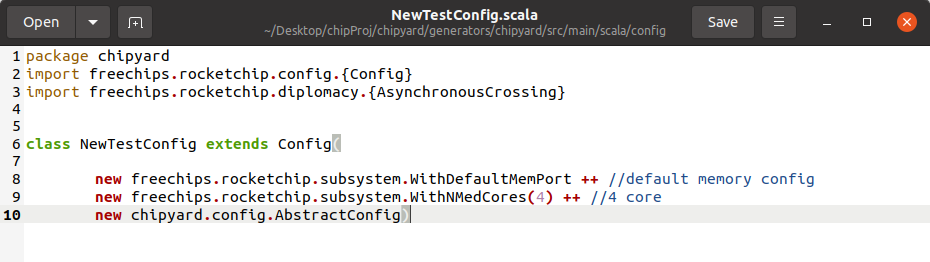
\includegraphics[width=0.7\linewidth]{./NewTestConfig.png}
  \caption{NewTestConfig.scala}
  \label{fig:newtestconfig}
\end{figure}

%%% Local Variables:
%%% mode: latex
%%% TeX-master: "../doc"
%%% End:
